\documentclass[a4paper]{article}

%% Language and font encodings
\usepackage[english]{babel}
\usepackage[utf8x]{inputenc}
\usepackage[T1]{fontenc}
\usepackage{parskip}

%% Sets page size and margins
\usepackage[a4paper,top=3cm,bottom=2cm,left=3cm,right=3cm,marginparwidth=1.75cm]{geometry}

%% Useful packages
\usepackage{amsmath}
\usepackage{graphicx}
\usepackage[colorinlistoftodos]{todonotes}
\usepackage[colorlinks=true, allcolors=blue]{hyperref}
\usepackage{tabu}
\usepackage{tikz}

\title{DD2360 Project}
\author{Victor Ähdel, Tim Olsson, Alex Sundström, Konrad Magnusson}

\begin{document}
\maketitle

\section{Introduction}

In this project we aim to replicate the results in \emph{N-Body Simulation of the Formation of the Earth-Moon System} \cite{simulation_paper}.
The paper is trying to simulate the giant impact hypothesis, which claims that the creation of our earth and moon stems from the collision of two earth sized planets.
This theory originated from the fact that the earth and moon share a lot of isotopes, however the moon has a lot less iron.
The replication is implemented using Cuda and OpenGL.
Our work amounted in the open-sourced code at \url{https://github.com/timsl/agp-grus}.




\subsection{Scope}

Due to the limited time frame of the project, we restrict ourselves to shorter runs than in the original article.
As the original authors ran some simulations for 720 hours while using 100k particles, it is simply infeasible for us to do the same.
Furthermore, we are not able to search the parameter space as extensively due to time constraints, so we might not necessarily end up with as good parameters as the original authors for the smaller number of particles.

\section{Methodology}

The implementation uses CUDA \cite{Cuda} for simulating the particles.
Rendering the simulation is achieved with OpenGL \cite{opengl}, using GLFW for the window management \cite{glfw}.

\subsection{Model}

We follow the model outlined in \cite{simulation_paper} but with a few modifications to enable completing the simulation in less time.
Their model is a normal n-body simulation, and all the particle interactions are summarized in `Table 2: Force function' in \cite{simulation_paper}.

\subsection{Initialization Of Planets}

The planets consist of two different types of particles, iron particles which form the inner core and silicate particles which form an outer shell. 
We begin by initializing the particles' positions by randomly sampling in spherical coordinates. 
For the inner core we sample from a spherical source. 
This is done by firstly uniformly sampling three numbers between 0 and 1, in equations 1-3 referred to as $\rho_1$, $\rho_2$, and $\rho_3$. 
After that we calculate the particles' positions using the following equations:

\begin{equation}
x = rsin\theta cos\phi = R\rho^{1/3}_{1}(1-\mu^{2})^{1/2}cos(2\pi\rho_{3})
\end{equation}
\begin{equation}
y = rsin\theta sin\phi = R\rho^{1/3}_{1}(1-\mu^{2})^{1/2}sin(2\pi\rho_{3})
\end{equation}
\begin{equation}
z = rcos\theta = R\rho^{1/3}_{1}\mu
\end{equation}

The outer shell we distribute the particles according to a random shell distribution. 
Similarly to the inner shell, we begin by uniformly sampling three numbers between 0 and 1, $\rho_1$, $\rho_2$, $\rho_3$ in equation 4-6. 
We then calculate the positions using the following equations:

\begin{equation}
x = rsin\theta cos\phi = [R^3_1 + (R^3_2 - R^3_1)\rho_1)]^{1/3}(1 - \mu^2)^{1/2}cos(2\pi\rho_3)
\end{equation}
\begin{equation}
y = rsin\theta sin\phi = [R^3_1 + (R^3_2 - R^3_1)\rho_1)]^{1/3}(1 - \mu^2)^{1/2}sin(2\pi\rho_3)
\end{equation}
\begin{equation}
z = rcos\theta = [R^3_1 + (R^3_2 - R^3_1)\rho]^{1/3}\mu
\end{equation}


As the simulations start after the collision, the initial particle velocities of the two planets are opposite of each other. 
The initial velocities of each particle has to take into account the impact and the rotational velocities as they were rotating around the Y axis. 
The rotational velocity is computed by firstly calculating the distance to the center of mass, followed by calculating the angle and finally adding the rotational velocity. 
The impact velocity is added to the x velocity as a factor of $+/- 3.2416 km/s$ depending on which planet the particle belongs to.

\begin{center}
$r = \sqrt{((x - \bar{x})^2 + (z - \bar{z})^2)}$ \\
$\theta = \arctan((z - \bar{z})/(x - \bar{x}))$ \\
$x_{velocity} = +/-3.2416 + omega*r_xz*sin(theta)$ \\
$y_{velocity} = -omega*r_xz*cos(theta)$ \\
\end{center}


\subsection{CUDA}

The most significant part of the computation that needs to be done for the simulation is in the force calculations between the particles.
Generally in n-body simulations each particle affects each other particle with for example gravity.
This implies that the computational complexity is $O(n^2)$.
While there are ways of reducing the computations necessary, the original paper claims to not do any such optimizations, in order to keep a maximal amount of accuracy in the simulation.
By extension, we do not perform any such optimizations either, and so that computation is by far the biggest bottleneck in achieving a performant simulation.

We therefore use CUDA in order to leverage more power for the n-body force calculations.
Our algorithm is loosely based on the examples in the Nvidia Gems book chapter 31 \cite{nvidia_gems}.
We started out without looking at the book by just computing the forces necessary by running one kernel per particle, which implies that we just need to iterate through every other particle in that kernel.
That code happened to do pretty much the same things as in the book, aside from the shared memory usage which afterwards was rather easy to add on.
The change affected the performance only very slightly though, probably due to how well modern GPGPU drivers cache things anyway when there is free shared memory to use.
Our code should therefore now do the same work as in the article, but it is not structured exactly the same.

In order to improve the performance of the code, we optimized the code by eliminating slow performing function calls with simpler ones.
The code bottlenecks were found using the profilers \verb|nvprof| and the NVIDIA Visual Profiler.
One necessary optimization was to eliminate all usages of \verb|pow()|, as that was seen to take a long time.
Normally such changes would seem to be a "micro-optimization", and you would prefer that the code remains as close to the mathematics as possible, but in this case it made too much of a difference.
It ended up approximately reducing the time needed for the n-body computations to a tenth of the original.

In addition, we also tried to reduce the amount of branching as much as possible by not having if-statements for the particle types as well as pre-computing common values.
The if-statements for the types can rather simply be replaced by indexing a property array with an enum that is based on the type of the particle.
We also compute all of the values that are necessary in all of the branches before branching anything, which will hopefully reduce cache issues related to branch misses, since those parts will always be done.
Furthermore, we do not do the if statements quite as in the original article, since that would incur more branches than necessary.
Instead, we branch in such a way that the common case where the particles are moving towards each other is not duplicated in different branches, and the logic was a bit simplified by multiplying with $KRP$ in all cases, but setting it to $1.0$ if it shouldn't be used.
By doing so we seemed to end up with a lot fewer branch-related performance issues.


\subsection{Camera}

In order to be able to move around the space and visualize the simulation from the best angle we needed a smooth and easily operated camera.
To that end, we implemented a camera that acts similar to how a spaceship might act, with controls like a first-person shooter.
We maintain three vectors at all times, a position vector and two direction vectors for forward and upwards.
For a rotation up or down we can take the cross product of the forward and upwards vector to recover a right-pointing vector, and rotate the forward and upwards vector about that axis.
Similarly, rotations left or right simply rotate the forward vector about the upwards vector.

\subsection{OpenGL}

To handle the visualization of the particles we used OpenGL\cite{opengl}. 
As a starting point a code skeleton of the GLFW verion of the OpenGL lab was used. 
To improve performance a sphere struct was created which handled the rendering. 
Beyond that instanced rendering and face culling was also added. 

\subsubsection{The Sphere Struct}
\label{sphere_struct}

The sphere struct holds it's own vertex array object (VAO) which in turn has two vertex array buffers (VBO). 
The first of these buffers is used for storing the vertices of the sphere and the second for the instanced rendering (see section \ref{instanced}). 
To create the vertices we use the same code as in the OpenGL labs \verb|GLUTSolidSphere| function. 
However since we only set up these vertices once and reuse them we save on performance.
When we close the application the struct will delete both the VBOs and the VAO. 

\subsubsection{Instanced Rendering}
\label{instanced}

To render all the particles we need to provide the GPU with the spheres vertices and a model-view-projection matrix. 
Doing this for every single particle does not scale very well since we need to make these OpenGL function calls on the CPU for every particle individually.
It would be better if all the relevant data was pushed to the GPU once and we issued a single call to render all the particles. 
Instanced rendering does exactly that. 

To achieve instanced rendering we use one large VBO which houses four floats and one unsigned integer for every particle. 
This is different from the recommended shader storage buffer object (SSBO) approach, where we can define the necessary data like structs, but it works quite well. 
The floats are the particles position in homogeneous coordinates and the integer the type of particle (used for deciding which color to render it with). 
This second VBO is as such of length $4 \times GL\_FLOAT + GL\_UNSIGNED\_INT$ times the number of particles. 
The type data (which is in the int) theoretically fits into just 2 bits (2 elements types, 2 planets), but we needed to align the data to a 32-bit boundary in order for the later parts in CUDA to work.
An illustration of the structure of this VBO can be seen in Figure \ref{instanced_figure}.
By adding a stride and offset with \verb|glVertexAttribPointer| and setting \verb|glVertexAttribDivisor| to one OpenGL will know that this is a instanced buffer. 

\begin{figure}
\centering

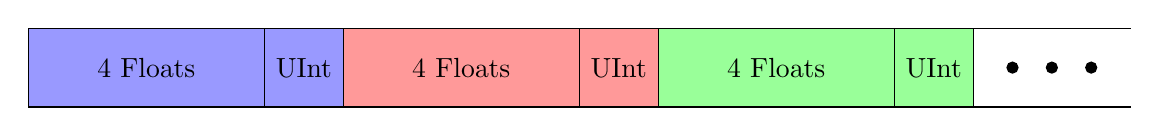
\begin{tikzpicture}

\filldraw[fill=blue!40!white, draw=black] (0,0) rectangle (3,1) node[pos=.5] {4 Floats};
\filldraw[fill=blue!40!white, draw=black] (3,0) rectangle (4,1) node[pos=.5] {UInt};
\filldraw[fill=red!40!white, draw=black] (4,0) rectangle (7,1) node[pos=.5] {4 Floats};
\filldraw[fill=red!40!white, draw=black] (7,0) rectangle (8,1) node[pos=.5] {UInt};
\filldraw[fill=green!40!white, draw=black] (8,0) rectangle (11,1) node[pos=.5] {4 Floats};
\filldraw[fill=green!40!white, draw=black] (11,0) rectangle (12,1) node[pos=.5] {UInt};

\draw (12,1) -- (14,1);
\filldraw (12.5,0.5) circle (2pt);
\filldraw (13,0.5) circle (2pt);
\filldraw (13.5,0.5) circle (2pt);
\draw (12,0) -- (14,0);

\end{tikzpicture}

\caption{Illustration of how the data is packed in the VBO used for the instanced rendering. 
The different colors indicate that the data belongs to a different instance of the spheres. 
Note that this illustration only shows the data needed for three spheres, when in fact the actual VBO is much larger.}
\label{instanced_figure}

\end{figure}

When we then render the particles we first update this large VBO. 
Then we compute a view-projection matrix which we send as a uniform to the OpenGL vertex shader. 
When\\ \verb|glDrawElementsInstanced| is called OpenGL will draw the same vertices stored in the first VBO but will step through the second VBO to find the position and type of the particle. 
In the vertex shader we have to define two new in paramters with thier own locations, one for a \verb|vec4| and one for a \verb|uint|. 
The \verb|vec4| is used for calculating the particles position and the \verb|uint| is sent to the fragment shader as an \emph{flat out} parameter, to indicate that it is an integer.  

Note that we issue more then one call on the CPU side for every render cycle because of the nature of the \verb|GLUTSolidSphere| code we based our rendering on.
The number of calls depends on how many "\emph{stacks}" the spheres have.
Even so the rendering is still very fast even as the number of particles start to scale to over 100,000. 

\subsubsection{Face Culling}

We turned on face culling by calling \verb|glEnable(GL_CULL_FACE)| and \verb|glCullFace(GL_BACK)| during the initialization of the program. 
Turning the face culling on provided an approximate $32$ percent performance boost to the OpenGL rendering. 

  

\subsection{Interop}

One bottleneck when programming GPUs is the transfer of memory between the CPU and the GPU. 
If we only are interested in the simulation then all the memory can stay on the GPU. 
However since we are also visualizing the particles in tandem with the simulation we have to move the new particle positions from the GPU to the CPU to prepare OpenGL to render them. 
Then we again have to send this data to the GPU where OpenGL can access it. 
With Interop we can let CUDA send the new positions to a OpenGL buffer directly, eliminating the intermediate transfer step. 
This can be a quite good speedup especially as the number of particles, and as such the memory requirements, grow. 

To achieve interoperability between OpenGL and CUDA we had to expose the Sphere structs (see \ref{sphere_struct}) VBO containing the positions and types to the CUDA kernel. 
First a \verb|cudaGraphicsResource| had to be created. 
To expose the VBO to this resource \verb|cudaGraphicsGLRegisterBuffer| was used, and then the resource was mapped with \verb|cudaGraphicsMapResources|. 
Finally, a pointer to the VBO was fetched with \verb|cudaGraphicsResourceGetMappedPointer|. 
After each update cycle this pointer was used to access the VBO and update the particles positions. 
This was done using some pointer math and required that the data types in the VBO was aligned to a 32-bit boundary. 

\section{Simulation Results}

\subsection{Parameters}
The simulation was very sensitive to the time step parameter. 
In the original report a timestep of $5.8117$ seconds was used \cite{simulation_paper}. 
However with such a large step size the particles were more likely to just scatter away. 
This is possibly because they then more often ended up penetrating both shells in a single update step, immediately being affected by large forces.
We had more success with a lower time step, which made more particle interactions start while they barely touched each other, which implies that the inner shells were less often penetrated as the first thing, and therefore the elastic forces were at play.
With the lower timestep, it also means that generally lower forces will be applied when particles start to collide, and the system stays more stable.

\subsection{Creation of the moon}
TODOTIM 

utveckling 100k partiklar, ingen måne, 

our simulation ended up seeming very reasonable, but we did not find the exact parameters that created a moon

here are nice images though::::


\section{Performance Results}
We used a computer with an i5-2500k CPU and an Nvidia GeForce GTX 960 GPU with 4GiB VRAM for the benchmarks.
As pretty much all the work is done on the GPU, the CPU will not be the bottleneck, and so it should not affect the measurements noticeably.
All the measurements here are averages of 64 update steps.

In table \ref{cudatime} the performance of the CUDA part is summarized.
It is there very visible that the time complexity is about $O(n^2)$, since each step down a row approximately quadruples the time.
We can also see that the optimal block size depends a bit on the choice of the number of particles.
For low number of particles, a block size of 256 might be optimal, while the more reasonably large simulations would like a block size of 1024.
We could not try out larger block sizes, as at that point the blocks run out of shared memory and the CUDA part stops working.
The standard deviations here are omitted for space since they scaled approximately the same as the time itself, and was consistently about a tenth of the time.
Most of the standard deviation appears to come from a few outliers, such as the first update step in each run which takes a significant higher amount of time (probably due to the GPU not having cached anything yet).
The same information is visible in figure \ref{cudatimeplot}, where the scaling is even more obvious.
Table \ref{nvprof} shows the relative time taken by the kernels for a run with 65536 particles, verifying that the force calculations take most of the time and the other kernels are negligible.

Table \ref{opengltime} summarizes the performance of the OpenGL part depending also on the number of particles.
There we can see that the time scales approximately linearly with the number of particles.

\begin{table}[ht]
\center
\begin{tabu} to \textwidth {r|rrrrrrrr}
  Particles &   8 &  16 & 32 &  64 & 128 & 256 & 512 &1024 \\
\hline
 1024 &     574 &    478 &    454 &    443 &    439 &    438 &    447 &    508 \\
 2048 &    1552 &    926 &    788 &    760 &    744 &    737 &    743 &    843 \\
 4096 &    5124 &   2631 &   1697 &   1582 &   1514 &   1483 &   1456 &   1626 \\
 8192 &   19724 &   9951 &   5084 &   4359 &   3968 &   3811 &   3711 &   3655 \\
16384 &   77976 &  39116 &  19784 &  18670 &  17437 &  17000 &  14660 &  14350 \\
32768 &  311170 & 155934 &  78569 &  77015 &  70697 &  68759 &  58424 &  57163 \\
65536 & 1248198 & 626355 & 314103 & 281629 & 259492 & 252709 & 234937 & 231091 \\
\end{tabu}
\caption{Mean update time (CUDA part). Columns are the block size. Times are in microseconds.}
\label{cudatime}
\end{table}

\begin{figure}[ht]
\center
\includegraphics[width=0.8\textwidth]{plot}
\caption{Plot of the mean update time (CUDA part), dependent on the number of particles and block size. Times are in microseconds. Both axes are in log 2.}
\label{cudatimeplot}
\end{figure}

\begin{table}[ht]
\center
\begin{tabu} to \textwidth {l|rr}
  Kernel & Time & \%\\
\hline
\texttt{calculate\_forces} & 57541 & 99.85\%\\
\texttt{apply\_forces} & 52 & 0.09\%\\
\texttt{update\_gl} & 31 & 0.06\%\\
\end{tabu}
\caption{\texttt{nvprof} results for the kernels that run each update. Average times for a run with 65536 particles. Times are in microseconds.}
\label{nvprof}
\end{table}

\begin{table}[ht]
\center
\begin{tabu} to \textwidth {r|rr}
Particles & Mean & Std.Dev. \\
\hline
  1024    &       428      &      428 \\
  2048    &       555      &      413 \\
  4096    &       833      &      556 \\
  8192    &      1274      &      681 \\
 16384    &      2280      &      805 \\
 32768    &      4108      &      894 \\
 65536    &      8155      &      912 \\
\end{tabu}
\caption{Display time (OpenGL part). Times are in microseconds.}
\label{opengltime}
\end{table}


\section{Discussion and Conclusion}

While we did not manage to recreate the moon in the exact manner as in the original article, we have succeeded in creating moon-like planets as a result of the collision.
Hence, we believe that the simulation method is very promising, and can certainly simulate this type of collision.

The usage of GPGPU methods for the simulation was certainly key to enable the program to perform efficiently enough for reasonably fast simulation and parameter searching.
The simulation could definitely not have been done if we could not make usage of our GPUs, as we would then need supercomputer-grade CPUs for the simulation to complete in a reasonable time frame.

It is as of yet unclear whether it was necessary to do the full $n^2$ particle computation, or if it might have been possible to use other optimizations while ending up with the same result.
It would be interesting to see if the simulation would still work well using hierarchical approaches with far-field approximations, that split the particles into groups and then approximate the forces against particles far away, instead of doing the all-pair version.

On the rendering side the most important optimization was the inclusion of instanced rendering.
For this specific application this provided enough of a boost that rendering a very large amount of particles became very easy.
Further optimizations are not very needed on our testing hardware since the larger bottleneck is in the simulation code.
However one thing that would improve the user experience would be to let the rendering and simulation be done on different threads. 
This would allow the user to manipulate the camera in a smooth fashion even when the simulation would dip below real time. 
To implement this in a proper manner triple buffering of the larger VBO mentioned in \ref{instanced} would be needed. 

\section{Contribution of each member}
The team members all did a similar amount of work.
We most often used pair programming and mutually discussed the code while actually writing it on the computers with the most comfortable CUDA environment, so the git log is very inaccurate as to our work split.

\bibliographystyle{apalike}
\bibliography{sample}

\end{document}